\documentclass[titlepage,a4paper,11pt]{article}
\usepackage{a4wide}
\usepackage[colorlinks=true,linkcolor=black,urlcolor=blue,bookmarksopen=true]{hyperref}
\usepackage{bookmark}
\usepackage{fancyhdr}
\usepackage[spanish]{babel}
% Default to the notebook output style

% Inherit from the specified cell style.

    \usepackage[T1]{fontenc}
    % Nicer default font (+ math font) than Computer Modern for most use cases
    \usepackage{mathpazo}

    % Basic figure setup, for now with no caption control since it's done
    % automatically by Pandoc (which extracts ![](path) syntax from Markdown).
    \usepackage{graphicx}
    % We will generate all images so they have a width \maxwidth. This means
    % that they will get their normal width if they fit onto the page, but
    % are scaled down if they would overflow the margins.
    \makeatletter
    \def\maxwidth{\ifdim\Gin@nat@width>\linewidth\linewidth
    \else\Gin@nat@width\fi}
    \makeatother
    \let\Oldincludegraphics\includegraphics
    % Set max figure width to be 100% of text width, for now hardcoded.
    \renewcommand{\includegraphics}[1]{\Oldincludegraphics[width=\maxwidth]{#1}}
    % Ensure that by default, figures have no caption (until we provide a
    % proper Figure object with a Caption API and a way to capture that
    % in the conversion process - todo).
    \usepackage{caption}
    \DeclareCaptionLabelFormat{nolabel}{}
    \captionsetup{labelformat=nolabel}

    \usepackage{adjustbox} % Used to constrain images to a maximum size 
    \usepackage{xcolor} % Allow colors to be defined
    \usepackage{enumerate} % Needed for markdown enumerations to work
    \usepackage{geometry} % Used to adjust the document margins
    \usepackage{amsmath} % Equations
    \usepackage{amssymb} % Equations
    \usepackage{textcomp} % defines textquotesingle
    % Hack from http://tex.stackexchange.com/a/47451/13684:
    \AtBeginDocument{%
        \def\PYZsq{\textquotesingle}% Upright quotes in Pygmentized code
    }
    \usepackage{upquote} % Upright quotes for verbatim code
    \usepackage{eurosym} % defines \euro
    \usepackage[mathletters]{ucs} % Extended unicode (utf-8) support
    \usepackage[utf8x]{inputenc} % Allow utf-8 characters in the tex document
    \usepackage{fancyvrb} % verbatim replacement that allows latex
    \usepackage{grffile} % extends the file name processing of package graphics 
                         % to support a larger range 
    % The hyperref package gives us a pdf with properly built
    % internal navigation ('pdf bookmarks' for the table of contents,
    % internal cross-reference links, web links for URLs, etc.)
    \usepackage{hyperref}
    \usepackage{longtable} % longtable support required by pandoc >1.10
    \usepackage{booktabs}  % table support for pandoc > 1.12.2
    \usepackage[inline]{enumitem} % IRkernel/repr support (it uses the enumerate* environment)
    \usepackage[normalem]{ulem} % ulem is needed to support strikethroughs (\sout)
                                % normalem makes italics be italics, not underlines
    

    
    
    % Colors for the hyperref package
    \definecolor{urlcolor}{rgb}{0,.145,.698}
    \definecolor{linkcolor}{rgb}{.71,0.21,0.01}
    \definecolor{citecolor}{rgb}{.12,.54,.11}

    % ANSI colors
    \definecolor{ansi-black}{HTML}{3E424D}
    \definecolor{ansi-black-intense}{HTML}{282C36}
    \definecolor{ansi-red}{HTML}{E75C58}
    \definecolor{ansi-red-intense}{HTML}{B22B31}
    \definecolor{ansi-green}{HTML}{00A250}
    \definecolor{ansi-green-intense}{HTML}{007427}
    \definecolor{ansi-yellow}{HTML}{DDB62B}
    \definecolor{ansi-yellow-intense}{HTML}{B27D12}
    \definecolor{ansi-blue}{HTML}{208FFB}
    \definecolor{ansi-blue-intense}{HTML}{0065CA}
    \definecolor{ansi-magenta}{HTML}{D160C4}
    \definecolor{ansi-magenta-intense}{HTML}{A03196}
    \definecolor{ansi-cyan}{HTML}{60C6C8}
    \definecolor{ansi-cyan-intense}{HTML}{258F8F}
    \definecolor{ansi-white}{HTML}{C5C1B4}
    \definecolor{ansi-white-intense}{HTML}{A1A6B2}

    % commands and environments needed by pandoc snippets
    % extracted from the output of `pandoc -s`
    \providecommand{\tightlist}{%
      \setlength{\itemsep}{0pt}\setlength{\parskip}{0pt}}
    \DefineVerbatimEnvironment{Highlighting}{Verbatim}{commandchars=\\\{\}}
    % Add ',fontsize=\small' for more characters per line
    \newenvironment{Shaded}{}{}
    \newcommand{\KeywordTok}[1]{\textcolor[rgb]{0.00,0.44,0.13}{\textbf{{#1}}}}
    \newcommand{\DataTypeTok}[1]{\textcolor[rgb]{0.56,0.13,0.00}{{#1}}}
    \newcommand{\DecValTok}[1]{\textcolor[rgb]{0.25,0.63,0.44}{{#1}}}
    \newcommand{\BaseNTok}[1]{\textcolor[rgb]{0.25,0.63,0.44}{{#1}}}
    \newcommand{\FloatTok}[1]{\textcolor[rgb]{0.25,0.63,0.44}{{#1}}}
    \newcommand{\CharTok}[1]{\textcolor[rgb]{0.25,0.44,0.63}{{#1}}}
    \newcommand{\StringTok}[1]{\textcolor[rgb]{0.25,0.44,0.63}{{#1}}}
    \newcommand{\CommentTok}[1]{\textcolor[rgb]{0.38,0.63,0.69}{\textit{{#1}}}}
    \newcommand{\OtherTok}[1]{\textcolor[rgb]{0.00,0.44,0.13}{{#1}}}
    \newcommand{\AlertTok}[1]{\textcolor[rgb]{1.00,0.00,0.00}{\textbf{{#1}}}}
    \newcommand{\FunctionTok}[1]{\textcolor[rgb]{0.02,0.16,0.49}{{#1}}}
    \newcommand{\RegionMarkerTok}[1]{{#1}}
    \newcommand{\ErrorTok}[1]{\textcolor[rgb]{1.00,0.00,0.00}{\textbf{{#1}}}}
    \newcommand{\NormalTok}[1]{{#1}}
    
    % Additional commands for more recent versions of Pandoc
    \newcommand{\ConstantTok}[1]{\textcolor[rgb]{0.53,0.00,0.00}{{#1}}}
    \newcommand{\SpecialCharTok}[1]{\textcolor[rgb]{0.25,0.44,0.63}{{#1}}}
    \newcommand{\VerbatimStringTok}[1]{\textcolor[rgb]{0.25,0.44,0.63}{{#1}}}
    \newcommand{\SpecialStringTok}[1]{\textcolor[rgb]{0.73,0.40,0.53}{{#1}}}
    \newcommand{\ImportTok}[1]{{#1}}
    \newcommand{\DocumentationTok}[1]{\textcolor[rgb]{0.73,0.13,0.13}{\textit{{#1}}}}
    \newcommand{\AnnotationTok}[1]{\textcolor[rgb]{0.38,0.63,0.69}{\textbf{\textit{{#1}}}}}
    \newcommand{\CommentVarTok}[1]{\textcolor[rgb]{0.38,0.63,0.69}{\textbf{\textit{{#1}}}}}
    \newcommand{\VariableTok}[1]{\textcolor[rgb]{0.10,0.09,0.49}{{#1}}}
    \newcommand{\ControlFlowTok}[1]{\textcolor[rgb]{0.00,0.44,0.13}{\textbf{{#1}}}}
    \newcommand{\OperatorTok}[1]{\textcolor[rgb]{0.40,0.40,0.40}{{#1}}}
    \newcommand{\BuiltInTok}[1]{{#1}}
    \newcommand{\ExtensionTok}[1]{{#1}}
    \newcommand{\PreprocessorTok}[1]{\textcolor[rgb]{0.74,0.48,0.00}{{#1}}}
    \newcommand{\AttributeTok}[1]{\textcolor[rgb]{0.49,0.56,0.16}{{#1}}}
    \newcommand{\InformationTok}[1]{\textcolor[rgb]{0.38,0.63,0.69}{\textbf{\textit{{#1}}}}}
    \newcommand{\WarningTok}[1]{\textcolor[rgb]{0.38,0.63,0.69}{\textbf{\textit{{#1}}}}}
    
    
    % Define a nice break command that doesn't care if a line doesn't already
    % exist.
    \def\br{\hspace*{\fill} \\* }
    % Math Jax compatability definitions
    \def\gt{>}
    \def\lt{<}
    % Document parameters
    \title{Avisos\_laborales\_y\_postulaciones}
    
    
    

    % Pygments definitions
    
\makeatletter
\def\PY@reset{\let\PY@it=\relax \let\PY@bf=\relax%
    \let\PY@ul=\relax \let\PY@tc=\relax%
    \let\PY@bc=\relax \let\PY@ff=\relax}
\def\PY@tok#1{\csname PY@tok@#1\endcsname}
\def\PY@toks#1+{\ifx\relax#1\empty\else%
    \PY@tok{#1}\expandafter\PY@toks\fi}
\def\PY@do#1{\PY@bc{\PY@tc{\PY@ul{%
    \PY@it{\PY@bf{\PY@ff{#1}}}}}}}
\def\PY#1#2{\PY@reset\PY@toks#1+\relax+\PY@do{#2}}

\expandafter\def\csname PY@tok@w\endcsname{\def\PY@tc##1{\textcolor[rgb]{0.73,0.73,0.73}{##1}}}
\expandafter\def\csname PY@tok@c\endcsname{\let\PY@it=\textit\def\PY@tc##1{\textcolor[rgb]{0.25,0.50,0.50}{##1}}}
\expandafter\def\csname PY@tok@cp\endcsname{\def\PY@tc##1{\textcolor[rgb]{0.74,0.48,0.00}{##1}}}
\expandafter\def\csname PY@tok@k\endcsname{\let\PY@bf=\textbf\def\PY@tc##1{\textcolor[rgb]{0.00,0.50,0.00}{##1}}}
\expandafter\def\csname PY@tok@kp\endcsname{\def\PY@tc##1{\textcolor[rgb]{0.00,0.50,0.00}{##1}}}
\expandafter\def\csname PY@tok@kt\endcsname{\def\PY@tc##1{\textcolor[rgb]{0.69,0.00,0.25}{##1}}}
\expandafter\def\csname PY@tok@o\endcsname{\def\PY@tc##1{\textcolor[rgb]{0.40,0.40,0.40}{##1}}}
\expandafter\def\csname PY@tok@ow\endcsname{\let\PY@bf=\textbf\def\PY@tc##1{\textcolor[rgb]{0.67,0.13,1.00}{##1}}}
\expandafter\def\csname PY@tok@nb\endcsname{\def\PY@tc##1{\textcolor[rgb]{0.00,0.50,0.00}{##1}}}
\expandafter\def\csname PY@tok@nf\endcsname{\def\PY@tc##1{\textcolor[rgb]{0.00,0.00,1.00}{##1}}}
\expandafter\def\csname PY@tok@nc\endcsname{\let\PY@bf=\textbf\def\PY@tc##1{\textcolor[rgb]{0.00,0.00,1.00}{##1}}}
\expandafter\def\csname PY@tok@nn\endcsname{\let\PY@bf=\textbf\def\PY@tc##1{\textcolor[rgb]{0.00,0.00,1.00}{##1}}}
\expandafter\def\csname PY@tok@ne\endcsname{\let\PY@bf=\textbf\def\PY@tc##1{\textcolor[rgb]{0.82,0.25,0.23}{##1}}}
\expandafter\def\csname PY@tok@nv\endcsname{\def\PY@tc##1{\textcolor[rgb]{0.10,0.09,0.49}{##1}}}
\expandafter\def\csname PY@tok@no\endcsname{\def\PY@tc##1{\textcolor[rgb]{0.53,0.00,0.00}{##1}}}
\expandafter\def\csname PY@tok@nl\endcsname{\def\PY@tc##1{\textcolor[rgb]{0.63,0.63,0.00}{##1}}}
\expandafter\def\csname PY@tok@ni\endcsname{\let\PY@bf=\textbf\def\PY@tc##1{\textcolor[rgb]{0.60,0.60,0.60}{##1}}}
\expandafter\def\csname PY@tok@na\endcsname{\def\PY@tc##1{\textcolor[rgb]{0.49,0.56,0.16}{##1}}}
\expandafter\def\csname PY@tok@nt\endcsname{\let\PY@bf=\textbf\def\PY@tc##1{\textcolor[rgb]{0.00,0.50,0.00}{##1}}}
\expandafter\def\csname PY@tok@nd\endcsname{\def\PY@tc##1{\textcolor[rgb]{0.67,0.13,1.00}{##1}}}
\expandafter\def\csname PY@tok@s\endcsname{\def\PY@tc##1{\textcolor[rgb]{0.73,0.13,0.13}{##1}}}
\expandafter\def\csname PY@tok@sd\endcsname{\let\PY@it=\textit\def\PY@tc##1{\textcolor[rgb]{0.73,0.13,0.13}{##1}}}
\expandafter\def\csname PY@tok@si\endcsname{\let\PY@bf=\textbf\def\PY@tc##1{\textcolor[rgb]{0.73,0.40,0.53}{##1}}}
\expandafter\def\csname PY@tok@se\endcsname{\let\PY@bf=\textbf\def\PY@tc##1{\textcolor[rgb]{0.73,0.40,0.13}{##1}}}
\expandafter\def\csname PY@tok@sr\endcsname{\def\PY@tc##1{\textcolor[rgb]{0.73,0.40,0.53}{##1}}}
\expandafter\def\csname PY@tok@ss\endcsname{\def\PY@tc##1{\textcolor[rgb]{0.10,0.09,0.49}{##1}}}
\expandafter\def\csname PY@tok@sx\endcsname{\def\PY@tc##1{\textcolor[rgb]{0.00,0.50,0.00}{##1}}}
\expandafter\def\csname PY@tok@m\endcsname{\def\PY@tc##1{\textcolor[rgb]{0.40,0.40,0.40}{##1}}}
\expandafter\def\csname PY@tok@gh\endcsname{\let\PY@bf=\textbf\def\PY@tc##1{\textcolor[rgb]{0.00,0.00,0.50}{##1}}}
\expandafter\def\csname PY@tok@gu\endcsname{\let\PY@bf=\textbf\def\PY@tc##1{\textcolor[rgb]{0.50,0.00,0.50}{##1}}}
\expandafter\def\csname PY@tok@gd\endcsname{\def\PY@tc##1{\textcolor[rgb]{0.63,0.00,0.00}{##1}}}
\expandafter\def\csname PY@tok@gi\endcsname{\def\PY@tc##1{\textcolor[rgb]{0.00,0.63,0.00}{##1}}}
\expandafter\def\csname PY@tok@gr\endcsname{\def\PY@tc##1{\textcolor[rgb]{1.00,0.00,0.00}{##1}}}
\expandafter\def\csname PY@tok@ge\endcsname{\let\PY@it=\textit}
\expandafter\def\csname PY@tok@gs\endcsname{\let\PY@bf=\textbf}
\expandafter\def\csname PY@tok@gp\endcsname{\let\PY@bf=\textbf\def\PY@tc##1{\textcolor[rgb]{0.00,0.00,0.50}{##1}}}
\expandafter\def\csname PY@tok@go\endcsname{\def\PY@tc##1{\textcolor[rgb]{0.53,0.53,0.53}{##1}}}
\expandafter\def\csname PY@tok@gt\endcsname{\def\PY@tc##1{\textcolor[rgb]{0.00,0.27,0.87}{##1}}}
\expandafter\def\csname PY@tok@err\endcsname{\def\PY@bc##1{\setlength{\fboxsep}{0pt}\fcolorbox[rgb]{1.00,0.00,0.00}{1,1,1}{\strut ##1}}}
\expandafter\def\csname PY@tok@kc\endcsname{\let\PY@bf=\textbf\def\PY@tc##1{\textcolor[rgb]{0.00,0.50,0.00}{##1}}}
\expandafter\def\csname PY@tok@kd\endcsname{\let\PY@bf=\textbf\def\PY@tc##1{\textcolor[rgb]{0.00,0.50,0.00}{##1}}}
\expandafter\def\csname PY@tok@kn\endcsname{\let\PY@bf=\textbf\def\PY@tc##1{\textcolor[rgb]{0.00,0.50,0.00}{##1}}}
\expandafter\def\csname PY@tok@kr\endcsname{\let\PY@bf=\textbf\def\PY@tc##1{\textcolor[rgb]{0.00,0.50,0.00}{##1}}}
\expandafter\def\csname PY@tok@bp\endcsname{\def\PY@tc##1{\textcolor[rgb]{0.00,0.50,0.00}{##1}}}
\expandafter\def\csname PY@tok@fm\endcsname{\def\PY@tc##1{\textcolor[rgb]{0.00,0.00,1.00}{##1}}}
\expandafter\def\csname PY@tok@vc\endcsname{\def\PY@tc##1{\textcolor[rgb]{0.10,0.09,0.49}{##1}}}
\expandafter\def\csname PY@tok@vg\endcsname{\def\PY@tc##1{\textcolor[rgb]{0.10,0.09,0.49}{##1}}}
\expandafter\def\csname PY@tok@vi\endcsname{\def\PY@tc##1{\textcolor[rgb]{0.10,0.09,0.49}{##1}}}
\expandafter\def\csname PY@tok@vm\endcsname{\def\PY@tc##1{\textcolor[rgb]{0.10,0.09,0.49}{##1}}}
\expandafter\def\csname PY@tok@sa\endcsname{\def\PY@tc##1{\textcolor[rgb]{0.73,0.13,0.13}{##1}}}
\expandafter\def\csname PY@tok@sb\endcsname{\def\PY@tc##1{\textcolor[rgb]{0.73,0.13,0.13}{##1}}}
\expandafter\def\csname PY@tok@sc\endcsname{\def\PY@tc##1{\textcolor[rgb]{0.73,0.13,0.13}{##1}}}
\expandafter\def\csname PY@tok@dl\endcsname{\def\PY@tc##1{\textcolor[rgb]{0.73,0.13,0.13}{##1}}}
\expandafter\def\csname PY@tok@s2\endcsname{\def\PY@tc##1{\textcolor[rgb]{0.73,0.13,0.13}{##1}}}
\expandafter\def\csname PY@tok@sh\endcsname{\def\PY@tc##1{\textcolor[rgb]{0.73,0.13,0.13}{##1}}}
\expandafter\def\csname PY@tok@s1\endcsname{\def\PY@tc##1{\textcolor[rgb]{0.73,0.13,0.13}{##1}}}
\expandafter\def\csname PY@tok@mb\endcsname{\def\PY@tc##1{\textcolor[rgb]{0.40,0.40,0.40}{##1}}}
\expandafter\def\csname PY@tok@mf\endcsname{\def\PY@tc##1{\textcolor[rgb]{0.40,0.40,0.40}{##1}}}
\expandafter\def\csname PY@tok@mh\endcsname{\def\PY@tc##1{\textcolor[rgb]{0.40,0.40,0.40}{##1}}}
\expandafter\def\csname PY@tok@mi\endcsname{\def\PY@tc##1{\textcolor[rgb]{0.40,0.40,0.40}{##1}}}
\expandafter\def\csname PY@tok@il\endcsname{\def\PY@tc##1{\textcolor[rgb]{0.40,0.40,0.40}{##1}}}
\expandafter\def\csname PY@tok@mo\endcsname{\def\PY@tc##1{\textcolor[rgb]{0.40,0.40,0.40}{##1}}}
\expandafter\def\csname PY@tok@ch\endcsname{\let\PY@it=\textit\def\PY@tc##1{\textcolor[rgb]{0.25,0.50,0.50}{##1}}}
\expandafter\def\csname PY@tok@cm\endcsname{\let\PY@it=\textit\def\PY@tc##1{\textcolor[rgb]{0.25,0.50,0.50}{##1}}}
\expandafter\def\csname PY@tok@cpf\endcsname{\let\PY@it=\textit\def\PY@tc##1{\textcolor[rgb]{0.25,0.50,0.50}{##1}}}
\expandafter\def\csname PY@tok@c1\endcsname{\let\PY@it=\textit\def\PY@tc##1{\textcolor[rgb]{0.25,0.50,0.50}{##1}}}
\expandafter\def\csname PY@tok@cs\endcsname{\let\PY@it=\textit\def\PY@tc##1{\textcolor[rgb]{0.25,0.50,0.50}{##1}}}

\def\PYZbs{\char`\\}
\def\PYZus{\char`\_}
\def\PYZob{\char`\{}
\def\PYZcb{\char`\}}
\def\PYZca{\char`\^}
\def\PYZam{\char`\&}
\def\PYZlt{\char`\<}
\def\PYZgt{\char`\>}
\def\PYZsh{\char`\#}
\def\PYZpc{\char`\%}
\def\PYZdl{\char`\$}
\def\PYZhy{\char`\-}
\def\PYZsq{\char`\'}
\def\PYZdq{\char`\"}
\def\PYZti{\char`\~}
% for compatibility with earlier versions
\def\PYZat{@}
\def\PYZlb{[}
\def\PYZrb{]}
\makeatother


    % Exact colors from NB
    \definecolor{incolor}{rgb}{0.0, 0.0, 0.5}
    \definecolor{outcolor}{rgb}{0.545, 0.0, 0.0}



    
    % Prevent overflowing lines due to hard-to-break entities
    \sloppy 
    % Setup hyperref package
    \hypersetup{
      breaklinks=true,  % so long urls are correctly broken across lines
      colorlinks=true,
      urlcolor=urlcolor,
      linkcolor=linkcolor,
      citecolor=citecolor,
      }
    % Slightly bigger margins than the latex defaults
    
    \geometry{verbose,tmargin=1in,bmargin=1in,lmargin=1in,rmargin=1in}
    
\pagestyle{fancy} 
\fancyhf{}
\fancyhead[L]{TP1 - Segundo cuatrimestre de 2019}
\fancyhead[R]{Organización de Datos - FIUBA}
\renewcommand{\headrulewidth}{0.4pt}
\fancyfoot[C]{\thepage}
\renewcommand{\footrulewidth}{0.4pt}  

\begin{document}
\begin{titlepage}
    \hfill\adjustimage{width=6cm}{logofiuba.jpg}
    \centering
    \vfill
    \Huge \textbf{Trabajo Práctico 2 \\ Machine Learning}
    \vskip2cm
    \Large [75.06/95.58] Organización de Datos\\
    Segundo cuatrimestre de 2019\\
    Grupo 40
    \vskip5cm
    \normalsize \begin{tabular}{  l  l  l }
      Nombre & Padrón & E-mail \\ \hline
      DAVEREDE, Agustin & 98.540 & agusdaverede@yahoo.com.ar \\
  	\end{tabular}
    \vfill
    Repositorio: https://github.com/Distance71/TP-OrgaDatos
    \vfill
\end{titlepage}
    
\tableofcontents % Índice general
\newpage

\hypertarget{introducciuxf3n}{%
\section{Resumen}\label{introducciuxf3n}}
En el presente trabajo se realizó un análisis predictivo basado en técnicas de \textit{Machine Learning}, a partir de datos referidos a publicaciones realizadas en la página 'ZonaProp' en el periodo de 2012 a 2016 en México.

En primer lugar se evaluó el set de datos provisto, cuyo precio se debería predecir, ponderandolo con el análisis efectuado en la primera entrega. Posteriormente, se realizó un preprocesamiento de los datos provistos por el set de entrenamiento utilizando diversas técnicas.

Finalmente, se llevaron a cabo predicciones basadas en los algoritmos de \textit{Machine Learning} seleccionados.

\section{Introducción}
En el presente trabajo se buscó determinar cual era el precio de un determinado grupo de propiedades con base en sus características, en adelante \textit{features}. Para lograrlo, se desarrollo un modelo, con base en diversos y múltiples métodos, partiendo de un set de datos, en adelante denominado set de entrenamiento, cuya información permitiría a un algoritmo llevar a cabo dicha predicción.

Entre los algoritmos que se decidieron utilizar para efectuar la tarea, se destacan, primero, algoritmos simples basados en la regresión lineal, a partir de un solo \textit{feature} -\textit{LinearRegressor}-. Además, por otro lado, se pueden destacar algoritmos más complejos empleados como \textit{Decision Tree}, \textit{Lasso}, \textit{ElasticNet}, \textit{Ridge Regression}, \textit{SVR}, \textit{SGD Regressor}, \textit{XGG Boost} y por último \textit{Random Forest}. El análisis puntual de cada uno se encontrará en los siguientes apartados.

\section{Análisis preliminar}
En un comienzo, a la hora de aplicar técnicas de \textit{Machine Learning}, se debe efectuar un procesamiento preliminar de los sets de datos con los que se cuenta. Esto se hace con el objetivo de facilitar la tarea del algoritmo, cuya entrada serán dichos datos. A tales efectos, se hace uso de diversos métodos y criterios, que se describirán a continuación.

En primer lugar, y esto surge del análisis efectuado en el primer trabajo practico, resultó que no será de relevancia considerar los siguientes ítems:

\begin{itemize}
	\item Id
	\item Título
	\item Descripción
	\item Dirección
	\item Idzona
	\item Lat
	\item Lng
\end{itemize}

La razón es que sobre los mismos no recae información que deseemos considerar relevante en un principio. Si bien es cierto que podría utilizarse como un contraste realmente valioso de los \textit{features} que si se desean emplear. Por ejemplo, la dirección podría ser empleada para determinar, en conjunto con latitud y longitud, o bien por si misma, si la información con la que se cuenta de provincia y ciudad para una determinada propiedad son fidedignas. Sin embargo, estos análisis de mayor profundidad, requieren de ciertos conocimientos que no son el principal abordamiento de la asignatura, y cuya puesta en practica requeriría de una carga de trabajo sustancial, y el posible uso de fuentes de datos externas. Otro ejemplo que parece interesante mencionar, es la incidencia que podría llegar a tener el uso de determinadas palabras o conjuntos de palabras sobre el consumidor, haciendo referencia al título y la descripción. De igual modo que el ejemplo previo, su utilización y puesta en valor supondría una tarea de interés si se pensará en fines comerciales.

\subsection{Análisis de relación entre sets de datos}
Lo siguiente que se efectuó fue un análisis sobre el grado de utilidad y correlación que tendría el set de datos de entrenamiento respecto del set de evaluación. Con este fin, se asumió el uso de dos parámetros de referencia. En primer lugar, se consideró un parámetro que representaría la sumatoría de diferencias:

\begin{equation}
A_{k} = \sum_{i=1}^{n values}\\ \left|(x_{i}/x_{t})-(y_{i}/y_{t})\right| * 100
\end{equation}

Donde $x_{i}$ e $y_{i}$ representan la aparición de esos valores únicos dentro de cada respectivo set de datos, siendo indistinto. A su vez, $x_{t}$ e $y_{t}$ representan el total de datos, que son 240k y 60k.

Por otro lado, se considero un parámetro que representa la relación entre los promedios de los datos de cada set:

\begin{equation}
B_{k} = ((\left|x_{mean}/y_{mean}\right|) - 1) * 100
\end{equation}

Se obtuvieron los siguientes datos:

\begin{table}[h]
	\begin{center}
		\begin{tabular}{|c|c|c|}
			\hline
	Categoría & Relación de items [$A_{k}$] & Relación de medias [$B_{k}$] \\ \hline
	Tipo de propiedad & 0,669 & -\\ \hline
	Ciudad & 4,557 & -\\ \hline
	Provincia & 2,001 & -\\ \hline
	Antiguedad & 0,450 & 0,369\\ \hline
	Habitaciones & 0,278 & 0,171 \\ \hline
	Garages & 0,216 & 0,047 \\ \hline
	Baños & 0,450 & 0,191 \\ \hline
	Metros cubiertos & - & 0,154 \\ \hline
	Metros totales & - & 0,206 \\ \hline
	Fecha por año & 0,551 &  4.3e-05 \\ \hline
	Gimnasio & 0,235 & 1,88 \\ \hline
	Usos multiples & 0,088 & 0,802 \\ \hline
	Piscina & 0,177 & 1,011 \\ \hline
	Escuelas cercanas & 0,365 & 0,411 \\ \hline
	Centros comerciales cercanos & 0,447 & 0,563 \\ \hline
\end{tabular}
\caption{Tabla de parámetros}
\label{tabla:sencilla}
\end{center}
\end{table}

De esto es posible deducir que los sets de datos de entrenamiento y evaluación comparten una naturaleza, en lo relativo a \textit{features} en cierto modo similar, ya que el promedio de los datos resultaba similar y la otra medida que nos daba una referencia más puntual también resultó similar, siendo la excepción más notable el caso de provincia y ciudad. 

Además, como puede observarse la tabla está incompleta. La razón de esto es que si bien es posible calcular el parámetro $A_{k}$ para metros cubiertos y totales, dicha medición no tendría valor, ya que se trata de \textit{features} de tipo \textit{float}. En lo que respecta al item $B_{k}$ de los \textit{features} Tipo de propiedad, Ciudad y Provincia, hay una razón por la que el mismo no fue calculado y es que al momento de efectuar este análisis no se habían empleado técnicas como \textit{one-hot encoding}, y los resultados obtenidos se consideraron suficientes para proseguir.

Por último, se incluirá una tabla que describe el set de datos de evaluación, que nos dará la pauta que podemos adentrarnos en efectuar dicha tarea, ya que contamos, al menos, con los Id.

\begin{table}[h]
	\begin{center}
		\begin{tabular}{|c|c|c|}
			\hline
			Parámetro & Aparición [\%] & Cantidad de diferentes \\
			\hline \hline
			Id & 100 & 60000 \\ \hline
			Tipo de propiedad & 99,99 & 22  \\ \hline
			Ciudad  & 99,86 & 576  \\ \hline
			Provincia & 99,93 & 32  \\ \hline
			Antiguedad & 82,14 & 72  \\ \hline
			Habitaciones & 90,62 & 10  \\ \hline
			Garages & 84,46 & 4  \\ \hline
			Baños & 89,07 & 4 \\ \hline
			Metros cubiertos & 92,84 & 424  \\ \hline
			Metros totales & 78,91 & 424  \\ \hline
			Fecha & 100 & 1828  \\ \hline
			Gimnasio & 100 & 2  \\ \hline
			Usos multiples & 100 & 2  \\ \hline
			Piscina & 100 & 2 \\ \hline
			Escuelas cercanas & 100 & 2 \\ \hline
			Centros comerciales cercanos & 100 & 2 \\ \hline
		\end{tabular}
		\caption{Datos set de evaluación}
		\label{tabla:sencilla}
	\end{center}
\end{table}

Con base en lo explicitado, se asumirá que es posible utilizar el set de entrenamiento como base para el algoritmo que nos permitirá realizar las predicciones sobre el set de evaluación. El siguiente paso fue efectuar una adaptación de los datos.

\subsection{Adaptación de los datos}
Llegado a este punto, nos encontramos en posición de poder comenzar a trabajar con los datos. Esta tarea se dividirá, en primer lugar, en la creación de nuevos \textit{features}, que permitan establecer mayores relaciones entre los datos suministrados y nos lleven a una mejor predicción. Luego, además, se encuentra la transformación de los datos con que ya se cuenta, de carácter categórico o texto, en un tipo que puedan interpretar los algoritmos basados en cálculo numérico -lo deseado en este trabajo-.

\subsubsection{Creación de nuevos \textit{features}}

En este apartado es de destacar que si bien consideramos una buena práctica el aprovechamiento de los \textit{features} como herramienta para permitir a los algoritmos una mayor profundización en menos tiempo, no se ha encontrado algo realmente destacable. Del trabajo practico Nº1 surge información que podría ser relevante para un análisis, pero mayormente, al menos a criterio de quien suscribe, orientado a un algoritmo de clasificación.
Hay excepciones a esto, como son el año y el mes de publicación de una propiedad, pero como se observó, esto no constituye en un parámetro que incida mayormente sobre el precio de una propiedad. Esta posibilidad queda abierta y se comenta como posible mejora en el futuro.

\subsubsection{Transformación de datos de tipo categoría}
Dada la naturaleza de los datos que pueden interpretar los algoritmos que se describan luego, es necesario efectuar transformaciones sobre los datos que no poseen ese carácter a fin de lograr poder utilizar esa información. Es por esto, que se ha optado por utilizar dos técnicas que nos facilitan la tarea. 
datos
La primera es denominada \textit{one-hot encoding}, y se basa en la creación de nuevas columnas en el set de datos a partir de los datos únicos que se posean en la categoría, y la colocación de un dato de tipo binario en cada celda, según corresponda esa fila o no a dicha categoría. Además, por otro lado, se ha decidido utilizar otra técnica que se conoce como \textit{label encoding}, que funciona de un modo similar, pero en lugar de crear una nueva columna por cada dato único de la esa categoría, transforma cada línea única de texto en un número y las reemplaza.

Esto concluye el análisis y tratamiento preliminar de los datos. 

\section{Análisis de la solución}
En lo referido a la solución, se buscó implementar una predicción que minimizara el error respecto de los datos reales. Esto se trató de lograr partiendo de la premisa de la utilización de más de un algoritmo, sin mayor profundización en un principio, para luego, con variaciones de los datos suministrados -parámetros del algoritmo- (mediante la utilización de técnicas de \textit{one-hot encoding} y \textit{label encoding}), lograr mejores resultados. Previo al detalle de cada uno, se expondrán técnicas y criterio de uso general para la resolución del problema.

\subsection{Técnicas empleadas}

\subsubsection{Boosting}
Esta técnica consiste en la utilización de más de un algoritmo en simultaneo para buscar lograr una mayor \textit{performance} final con base en el trabajo en conjunto.

Lo cierto es que, por una cuestión de capacidad de trabajo y tiempo, no se llego a lograr implementar una solución que resultara conveniente, a partir de esta técnica. Solo se hicieron uso de los algoritmos de \textit{XGB Boost} y \textit{Random Forest} que emplean esta técnica. Luego, es una tarea que quedará pendiente de evaluación en posibles mejoras.

\subsubsection{Cross-Validation}
Consiste en la utilización un set de datos menor al de entrenamiento para llevar a cabo la etapa de entrenamiento del algoritmo, y la posterior validación del modelo utilizando el conjunto de datos restantes del mismo. Esto se hace con el objetivo de llegar a validar el modelo empleado. Además, una extensión interesante de este concepto resulta ser el la escalabilidad de un modelo basado en datos iniciales y su posterior incrementación.

Esta practica fue llevada a cabo.

\subsection{Algoritmos empleados}
Como se mencionó en apartados previos, se hizo uso de diversos algoritmos con su estructura e hiper parámetros por defecto. A su vez, se indago con mayor profundidad en aquellos cuyos resultados fueron de mayor conveniencia. Los mismos serán descriptos con mayor detalle en este apartado.

\subsubsection{Linear Regression}
La regresión lineal simple consiste en la generación de un modelo, a partir de los datos que mejor ajustan a una recta, con base en los datos suministrados en el set de entrenamiento. Una vez constituido el modelo, solo se predice cual es el valor que mejor ajustará a dicha recta con el nuevo punto. Este modelo es muy simple y no permite contemplar todos los \textit{features} que se poseen. Luego, solo nos sirve como una primera aproximación que no tendrá más valor salvo como caso de prueba.

\subsubsection{Decision Tree Regression}
Se trata de un modelo no paramétrico y supervisado que se encarga de predecir el valor objetivo a través de un algoritmo basado en la decisión de reglas simples basadas en las \textit{features} del set de datos.

Su fortaleza radica en su simplicidad, en que se requieren pocos datos para llegar a entrenar al algoritmo y en que permite la posibilidad de poder analizar datos de distinto tipo (incluyendo datos de tipo categoría), característica poco frecuente en este tipo de algoritmos. Por otro lado, su fortaleza es también su debilidad, ya que una variación mínima en el set de datos puede ocasionar que se produzcan grandes variaciones en el resultado obtenido. Otra desventaja resulta ser su capacidad de representar adecuadamente la información suministrada por el set de datos. Esto se conoce como \textit{overfitting}.


\subsubsection{Lasso y Elastic Net Regressor}
Se llegó a este algoritmo consultando diversas posibilidades en la web. Se trata de modelos \textit{sparse} caracterizados por el concepto de proyección de una matriz, con el calculo progresivo de ciertos coeficientes. No se indago más debido a que los resultados no fueron de interés.

\subsubsection{Ridge Regressor}
Se trata de un algoritmo que busca minimizar la suma de los cuadrados residuales -concepto matemático- mediante la imposición de una corrección por parámetro, buscando aproximarse a los datos. Su utilización no resultó de utilidad.

\subsubsection{SGD Regressor}
Este algoritmo en principio revistió un gran interés, ya que es de los pocos suministrados por la biblioteca \textit{scikit} que posee la capacidad de ser incremental. Es decir, se pueden ir agregando datos al modelo una vez entrenado, y este llevará a cabo un reajuste. Esta característica es conocida como \textit{feature scaling}. Su principal fortaleza, además, reviste en la eficiencia, lo que permite utilizarlo en grandes conjunto de datos, del orden de $10^{5}$ -según documentación-. Por otro lado, la desventaja que posee es la dificultad que conlleva fijar los hiper parámetros que el mismo requiere para lograr trabajar con exactitud.

Se hicieron dos pruebas con el mismo, logrando una significa mejora en la segunda evaluación de Kaggle, pero aún así no fue el mejor resultado.
\subsubsection{XGB Boost Regressor}
Se seleccionó este algoritmo con base en el consejo de un compañero que cursó la asignatura en un cuatrimestre previo, ya que el mismo posee una alta aceptación en el entorno de \textit{Machine Learning}.

Su principal fortaleza radica en la eficiencia, originalmente escrito en C++ y multi-core, su adaptabilidad y el hecho de que es posible personalizar su funcionamiento de un modo muy completo con base en diversos parámetros internos. Su utilización arrojó resultados interesantes, y sería recomendable su profundización en un próximo trabajo.
\subsubsection{SVR Regressor}

Este algoritmo fue seleccionado con base en el criterio suministrado por [4], haciendo referencia a la documentación, ya que el set de datos de evaluación se encuentra en el límite de dicho criterio. Desafortunadamente, su corrida no produjó resultados en el lapso de 8hs. Luego, se decidió abandonar su utilización.

\subsubsection{Random Forest Regressor}
Finalmente, llegamos al algoritmo que arrojó los mejores resultados.

Este algoritmo es un caso particular de un algoritmo de decisión, que incorpora el algoritmo de arboles aleatorios y el método de arboles extra. La principal característica del algoritmo es incorporar la aleatoriedad como herramienta para mitigar la varianza del bosque. Esto se logra tomando ciertos datos en la construcción de cada árbol y estructurándolos considerando el mejor orden asociados a las \textit{features}, de modo optimizar su relación de causalidad -correlación- en la posterior predicción.

Con respecto a los hiper parámetros, se modificó principalmente el referido a la cantidad de estimadores, obteniendo progresivamente mejores resultados. No se siguió aumentando el número, ya que la computadora empleada para la tarea, no lo permitió. Sin embargo, si se hicieron pruebas automatizadas con base en la cantidad de estimadores -\textit{trees}-.

\pagebreak

\section{Resultados obtenidos y análisis}
En el gráfico que se observa a continuación se llega a denotar el conjunto de resultados obtenidos, según el puntaje de Kaggle:

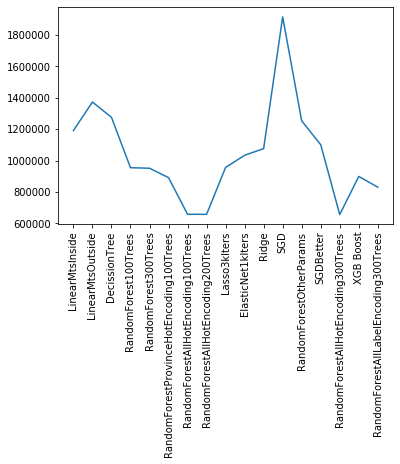
\includegraphics{Comparativa.png}

\subsection{Análisis de los resultados}
De los resultados obtenidos se puede llegar a la conclusión de que \textit{Random Forest} es el mejor algoritmo para este caso, con los parámetros testeados. Más allá de este hecho evidente lo cierto es que analizar en conjunto tantos algoritmos no resulta en una tarea sencilla, en especial cuando llegar a comprender en profundidad cada uno de ellos tampoco lo es. Sin embargo, si se puede hacer una evaluación de las mejoras notadas tras la incorporación de técnicas de modelado preliminares del set de datos, ya que aquí es donde se observó el mayor cambio en los resultados, más allá de lo arrojado debido a la especificidad propia de cada algoritmo. Una vez incorporados los \textit{features} de ciudad y provincia, se puede notar una significa mejora. Esto es razonable y consistente con lo observado en el trabajo practico previo, ya que esta información, la ubicación, incidía significativamente sobre los precios.

Otra mejora significativa se llegó a notar tras modificar los hiper parámetros de los algoritmos que se consideraron de mayor potencial. Esto es consistente, ya que ellos emplean estos datos para poder llevar a cabo las predicciones.

\section{Conclusiones}
El presente trabajo resultó de particular interés para nuestra formación profesional, permitiendo proporcionarnos un primer acercamiento a dos ramas de la informática que revisten muchas posibilidades y con potencial de crecimiento. Se trata de \textit{big data} y \textit{machine learning}. A su vez, se ha podido desarrollar un criterio analítico en la consideración de diversos algoritmos para la resolución de un problema.

Finalmente, vale destacar que tuvimos la oportunidad de participar de una practica basada en el empleo de datos reales y en la posibilidad de crecer como curso partiendo de la puesta en conjunto de los resultados, motivándonos a mejorar.

\subsection{Posibles mejoras}
En apartados previos, se ha mención a algunas mejoras que podrían considerar en un futuro. Además, valdría la pena mencionar que el set de datos provisto nos da la posibilidad de llevar a cabo una gran diversidad de análisis, con potencialidad productivo para Zonaprop, individualmente, y para el mercado inmobiliario en su conjunto. Para el primero, permitiendole profundizar el análisis más allá de poder predecir como se comportará económicamente el mercado, incorporando las ideas que podrían motivar mas al consumidor y a quien utilicen sus servicios. Para el segundo, pudiendo llegar a tener una referencia de considerable.

Además, se considera que sería posible profundizar más el uso de estos algoritmos, llegando a emplear tal vez otras técnicas y obtener mejores resultados.

Finalmente, es de interés considerar que se podrían efectuar más filtrados preeliminares a los datos que ya se poseen, considerando más categorias e incluso la diferencia que se llega a apreciar entre los datos de entrenamiento y evaluación en lo referido a ubicación (ciudad y provincia). Se hizo mención a esto en un apartado previo.

\section{Referencias consultadas}
[1] Luis Argerich, Apunte del Curso.

[2] Geron Aurelien, Hands‑On Machine Learning with Scikit‑Learn, Keras, and TensorFlow, Oreilly, 2017.

[3] $https://towardsdatascience.com/data-handling-using-pandas-machine-learning-in-real-life-be76a697418c$

[4] $https://scikit-learn.org/stable/tutorial/machine_learning_map/index.html$

[5] $https://medium.com/analytics-vidhya/building-a-machine-learning-model-to-predict-the-price-of-the-car-bc51783ba2f3$

[6] $https://nthu-datalab.github.io/ml/labs/05_Regularization/05_Regularization.html$

[7] $https://medium.com/@contactsunny/label-encoder-vs-one-hot-encoder-in-machine-learning-3fc273365621$
\end{document}\\
